%
% ---------------------------------------------------------------
% Copyright (C) 2012-2018 Gang Li
% ---------------------------------------------------------------
%
% This work is the default powerdot-tuliplab style test file and may be
% distributed and/or modified under the conditions of the LaTeX Project Public
% License, either version 1.3 of this license or (at your option) any later
% version. The latest version of this license is in
% http://www.latex-project.org/lppl.txt and version 1.3 or later is part of all
% distributions of LaTeX version 2003/12/01 or later.
%
% This work has the LPPL maintenance status "maintained".
%
% This Current Maintainer of this work is Gang Li.
%
%

\documentclass[
 size=14pt,
 paper=smartboard,  %a4paper, smartboard, screen
 mode=present, 		%present, handout, print
 display=slides, 	% slidesnotes, notes, slides
 style=tuliplab,  	% TULIP Lab style
 pauseslide,
 fleqn,leqno]{powerdot}


\usepackage{cancel}
\usepackage{caption}
\usepackage{stackengine}
\usepackage{smartdiagram}
\usepackage{attrib}
\usepackage{amssymb}
\usepackage{amsmath} 
\usepackage{amsthm} 
\usepackage{mathtools}
\usepackage{rotating}
\usepackage{graphicx}
\graphicspath{{figures/}}
\usepackage{boxedminipage}
\usepackage{rotate}
\usepackage{calc}
\usepackage[absolute]{textpos}
\usepackage{psfrag,overpic}
\usepackage{fouriernc}
\usepackage{pstricks,pst-3d,pst-grad,pstricks-add,pst-text,pst-node,pst-tree}
\usepackage{moreverb,epsfig,subfigure}
\usepackage{color}
\usepackage{booktabs}
\usepackage{etex}
\usepackage{breqn}
\usepackage{multirow}
\usepackage{natbib}
\usepackage{bibentry}
\usepackage{gitinfo2}
\usepackage{siunitx}
\usepackage{nicefrac}
%\usepackage{geometry}
%\geometry{verbose,letterpaper}
\usepackage{media9}
\usepackage{animate}
%\usepackage{movie15}
\usepackage{auto-pst-pdf}

\usepackage{breakurl}
\usepackage{fontawesome}
\usepackage{xcolor}
\usepackage{multicol}



\usepackage{verbatim}
\usepackage[utf8]{inputenc}
\usepackage{dtk-logos}
\usepackage{tikz}
\usepackage{adigraph}
%\usepackage{tkz-graph}
\usepackage{hyperref}
%\usepackage{ulem}
\usepackage{pgfplots}
\usepackage{verbatim}
\usepackage{fontawesome}


\usepackage{todonotes}
% \usepackage{pst-rel-points}
\usepackage{animate}
\usepackage{fontawesome}

\usepackage{listings}
\lstset{frameround=fttt,
frame=trBL,
stringstyle=\ttfamily,
backgroundcolor=\color{yellow!20},
basicstyle=\footnotesize\ttfamily}
\lstnewenvironment{code}{
\lstset{frame=single,escapeinside=`',
backgroundcolor=\color{yellow!20},
basicstyle=\footnotesize\ttfamily}
}{}


\usepackage{hyperref}
\hypersetup{ % TODO: PDF meta Data
  pdftitle={Presentation Title},
  pdfauthor={Gang Li},
  pdfpagemode={FullScreen},
  pdfborder={0 0 0}
}


% \usepackage{auto-pst-pdf}
% package to show source code

\definecolor{LightGray}{rgb}{0.9,0.9,0.9}
\newlength{\pixel}\setlength\pixel{0.000714285714\slidewidth}
\setlength{\TPHorizModule}{\slidewidth}
\setlength{\TPVertModule}{\slideheight}
\newcommand\highlight[1]{\fbox{#1}}
\newcommand\icite[1]{{\footnotesize [#1]}}

\newcommand\twotonebox[2]{\fcolorbox{pdcolor2}{pdcolor2}
{#1\vphantom{#2}}\fcolorbox{pdcolor2}{white}{#2\vphantom{#1}}}
\newcommand\twotoneboxo[2]{\fcolorbox{pdcolor2}{pdcolor2}
{#1}\fcolorbox{pdcolor2}{white}{#2}}
\newcommand\vpspace[1]{\vphantom{\vspace{#1}}}
\newcommand\hpspace[1]{\hphantom{\hspace{#1}}}
\newcommand\COMMENT[1]{}

\newcommand\placepos[3]{\hbox to\z@{\kern#1
        \raisebox{-#2}[\z@][\z@]{#3}\hss}\ignorespaces}

\renewcommand{\baselinestretch}{1.2}


\newcommand{\draftnote}[3]{
	\todo[author=#2,color=#1!30,size=\footnotesize]{\textsf{#3}}	}
% TODO: add yourself here:
%
\newcommand{\ranliu}[1]{\draftnote{cyan}{RLiu:}{#1}}
\newcommand{\gangli}[1]{\draftnote{blue}{GLi:}{#1}}
\newcommand{\shaoni}[1]{\draftnote{green}{sn:}{#1}}
\newcommand{\rlMarker}
{\todo[author=RLiu,size=\tiny,inline,color=cyan!40]
	{Ran Liu has worked up to here.}}
\newcommand{\gliMarker}
	{\todo[author=GLi,size=\tiny,inline,color=blue!40]
	{Gang Li has worked up to here.}}
\newcommand{\snMarker}
	{\todo[author=Sn,size=\tiny,inline,color=green!40]
	{Shaoni has worked up to here.}}

%%%%%%%%%%%%%%%%%%%%%%%%%%%%%%%%%%%%%%%%%%%%%%%%%%%%%%%%%%%%%%%%%%%%%%%%
% title
% TODO: Customize to your Own Title, Name, Address
%
\title{Disaster Tweets Prediction Using BERT}
\author{
Ran Liu
\\
\\Institute of Information Engineering
\\Chinese Academy of Sciences
}
\date{November 8, 2022}


% Customize the setting of slides
\pdsetup{
% TODO: Customize the left footer, and right footer
%rf=\href{http://www.tulip.org.au}{
%Last Changed by: \textsc{\gitCommitterName}\ \gitVtagn-\gitAbbrevHash\ (\gitAuthorDate)
%},
rf=\href{http://www.tulip.org.au}{
	Last Changed by: \textsc{\gitCommitterName}\ \gitAbbrevHash\ (\gitAuthorDate)
},
cf={Disaster Tweets Prediction Using BERT},
}


\begin{document}

\maketitle

%\begin{slide}{Overview}
%\tableofcontents[content=sections]
%\end{slide}



\begin{slide}[toc=,bm=]{Overview}
\tableofcontents[content=currentsection,type=1]
\end{slide}


\section{Problem Definition}


\begin{slide}{Disaster Tweets Prediction}
\begin{itemize}
	\item
	\smallskip
	Twitter has become an important communication channel in times of \textcolor{orange}{emergency}.
	\bigskip
	\item
	\smallskip
	But, it’s not always clear whether a person’s words are actually announcing a disaster.
\end{itemize}

\bigskip
	
%\begin{center}
	\twotonebox{\rotatebox{90}{e.g.}}{\parbox{.95\textwidth}
		{	\smallskip  \smallskip 
			LOOK AT THE SKY LAST NIGHT IT WAS ABLAZE!
			\begin{itemize}
				\item The author explicitly uses the word “ABLAZE” which is related to disaster.
				\item But it is an exaggerated expression.
			\end{itemize}
	}}


\end{slide}


\begin{slide}{Problem Description}
\twotonebox {\rotatebox{90}{Defn}}{\parbox{.88\textwidth}
{	\smallskip  \smallskip 
{Given a set of \textcolor{orange}{labeled} data which we will use to train a \textcolor{orange}{classifier} and use it to predict whether a tweet is about disaster or not.
\begin{itemize}
\item
The training set was collected from Twitter
\item
It has been labeled manually.
\item
A binary classification problem.
\item
F1 score is evaluation metric.
\end{itemize}
}
}}

\vspace{1.5cm}


\end{slide}



\section{Related Work and Challenges}



\begin{slide}{Related Work - Text Classification}
\begin{itemize}
\item
Existing Methods - \textcolor{orange}{Rule-Based Methods}

\begin{itemize}
\item
Rule-based methods classify text into different categories using a set of pre-defined rules.
\end{itemize}
\vspace{1cm}
\twocolumn[
\savevalue{lfrheight}=5cm,
\savevalue{lfrprop}={
linestyle=solid,framearc=.2,linewidth=1pt},
rfrheight=\usevalue{lfrheight},
rfrprop=\usevalue{lfrprop}
]{
	\smallskip \smallskip
Disadvantages
\begin{itemize}
\item
\smallskip
Require a deep domain knowledge.

\item
\smallskip
Require a lot of manpower and time. 

\item
\smallskip
When facing a new problem, previous rules may become useless.
\end{itemize}
}
{
	\smallskip \smallskip
Advantages
\begin{itemize}
\item
\smallskip
Fast

\item
\smallskip
Easy

\item
\smallskip
Interpretable
\end{itemize}
}
\end{itemize}

\end{slide}



\begin{slide}[toc=,bm=]{Related Work - Text Classification}

\begin{itemize}
\item
Existing Methods - \textcolor{orange} {Traditional Machine Learning (Statistical methods)}

\begin{itemize}
\item
Naïve Bayes, Support Vector Machines, Hidden Markov Model,  Random Forests...

\end{itemize}
\bigskip
\twocolumn[
\savevalue{lfrheight}=5cm,
\savevalue{lfrprop}={
linestyle=solid,framearc=.2,linewidth=1pt},
rfrheight=\usevalue{lfrheight},
rfrprop=\usevalue{lfrprop}
]{ \smallskip \smallskip
Disadvantages
\begin{itemize}
\item
\smallskip
Reliance on the handcrafted features.

\item
\smallskip
Cannot take full advantage of large training data because the features are pre-defined.

\end{itemize}
}{ \smallskip \smallskip
Advantages
\begin{itemize}
\item
\smallskip
More accurate than rule-based methods.

\end{itemize}
}
\end{itemize}
\end{slide}


\begin{slide}[toc=,bm=]{Related Work - Text Classification}
	
	\begin{itemize}
		\item
		Existing Methods - \textcolor{orange} {Deep Learning}
		
		\begin{itemize}
			\item
			Convolutional Neural Network, Long Short-Term Memory Network...
			
		\end{itemize}
		\bigskip
		\twocolumn[
		\savevalue{lfrheight}=5cm,
		\savevalue{lfrprop}={
			linestyle=solid,framearc=.2,linewidth=1pt},
		rfrheight=\usevalue{lfrheight},
		rfrprop=\usevalue{lfrprop}
		]{ \smallskip \smallskip
			Disadvantages
			\begin{itemize}
				\item
				\smallskip
				Reliance on large amount of training data.
				
				\item
				\smallskip
				Weak Interpretability.
				
			\end{itemize}
		}{ \smallskip \smallskip
			Advantages
			\begin{itemize}
				\item
				\smallskip
				Capture deep contexual features.
				
				\item
				\smallskip
				Greatly improve accuracy.
				
			\end{itemize}
		}
	\end{itemize}
	
\end{slide}


\begin{slide}{Challenges}
%Challenges (1)
\begin{itemize}
\item
How to capture deep features?

\begin{itemize}
\item
Models should have the ability to capture deep features.

\item
Generalization of models need to be improved.
\end{itemize}
\end{itemize}


\end{slide}

\begin{slide}[toc=,bm=]{Challenges}

\begin{itemize}
\item
Limited dataset.

\begin{itemize}
\item
Cannot train a model from scratch.

\item
Although dataset is small, performance of model still needs to meet the requirements.

\end{itemize}
\end{itemize}

\end{slide}



\section{Dataset}


\begin{slide}{Data Details}
%Step One - Group Feature Extraction}
\bigskip \bigskip \bigskip
\begin{table}[htbp]
	\setlength{\abovecaptionskip}{0pt}
	\setlength{\belowcaptionskip}{10pt}
	\centering
	\caption{Data structure}
	
	\begin{tabular}{ll}
		\hline
		Term                 & Example     \\
		\hline
		id     & 210                \\
		keyword          & airplain accident                         \\
		location         & Eagle Pass, Texas           \\
		text   & A Cessna airplane accident in Mexico...            \\
		label              & 1                   \\
		\hline
	\end{tabular}
\end{table}

\end{slide}



\begin{slide}{Data Statistics}
%Step Two - Outlying Degree Scoring
\bigskip \bigskip
\begin{itemize}
	\item
	Number of each label in training set.
\end{itemize}
\begin{table}[htbp]
	\setlength{\abovecaptionskip}{0pt}
	\setlength{\belowcaptionskip}{10pt}
	\centering
	\caption{Number of each label}
	
	\begin{tabular}{cc}
		\hline
		    label             & Number     \\
		\hline
		1     & 3721                \\
		 0          & 3892                        \\
		\hline
		total  &  7613 \\
				\hline
	\end{tabular}
\end{table}

\end{slide}



\begin{slide}[toc=,bm=]{Data Statistics}
	%Step Two - Outlying Degree Scoring
	\begin{itemize}
		\item
		Character length of text in training set.
			\begin{itemize}
			\item
			max: 157 \ \ \ \ \ min: 7
		\end{itemize}
	\end{itemize}


	\begin{figure}
		\centering
		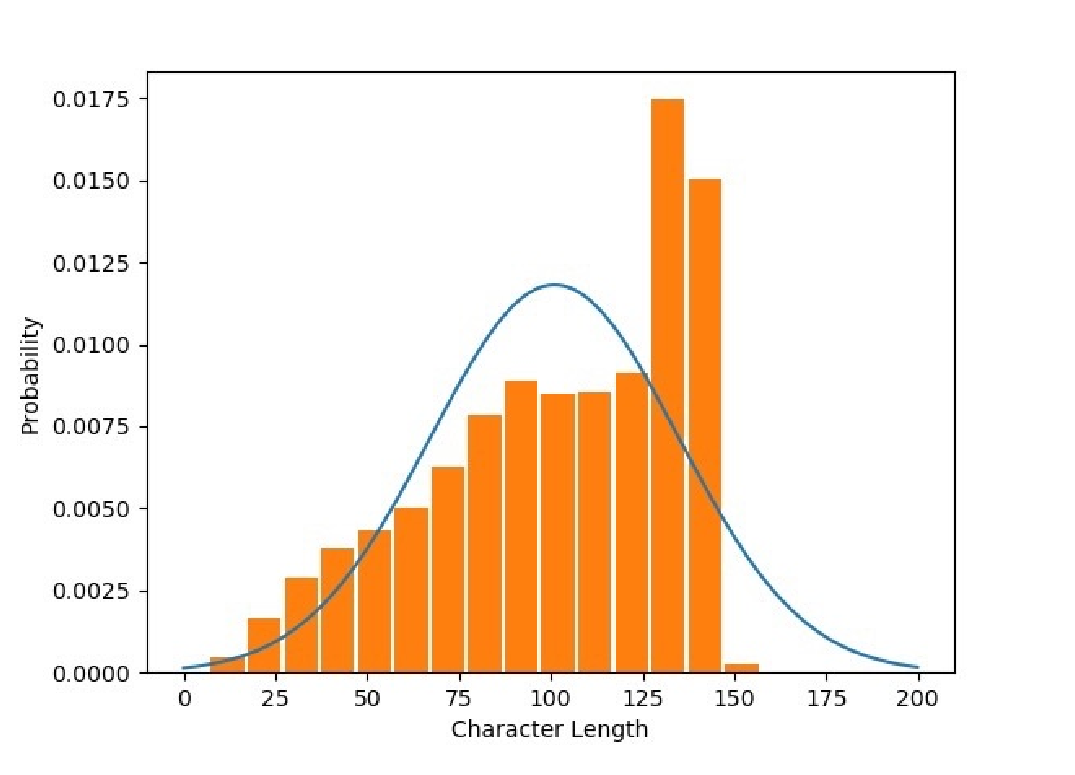
\includegraphics[scale=0.6]{character dist.eps}
		\caption{Distribution of Character Length}
	\end{figure}
\end{slide}



\begin{slide}[toc=,bm=]{Data Statistics}
	%Step Two - Outlying Degree Scoring
	\begin{itemize}
		\item
		Token length of text in training set.
		\begin{itemize}
			\item
			max: 84 \ \ \ \ \ min: 3
		\end{itemize}
	\end{itemize}
	
	
	\begin{figure}
		\centering
		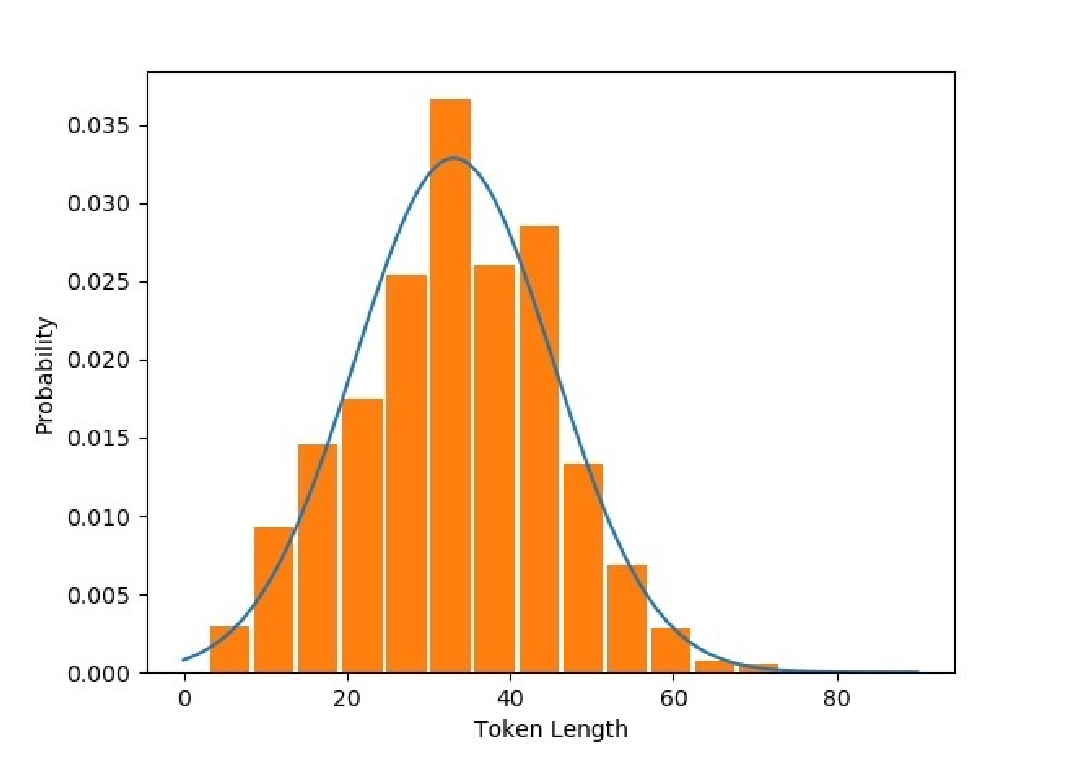
\includegraphics[scale=0.6]{token dist.eps}
		\caption{Distribution of Token Length}
	\end{figure}
	
\end{slide}



\section{Methodology}

\begin{slide}{Input Format}
	

		\begin{itemize}
			\item
			Original text: \\
			Three people died from the heat wave so far.
			\item
			Input format: 
			\begin{itemize}
				\item
				token vector: \\
				$[\ 101,\ 2093,\ 2111,\ 2351,\ 2013,\ 1996,\ 3684,\ 4400,\ 2061,\ 2521,\ 102,\ 0,\ 0,\ 0,\ ...\ ]$
				\item
				mask vector: \\
				$[\ 1,\ 1,\ 1,\ 1,\ 1,\ 1,\ 1,\ 1,\ 1,\ 1,\ 1,\ 0,\ 0,\ 0,\ ...\ ]$
				\item
				segment vector: \\
				$[\ 0,\ 0,\ 0,\ 0,\ 0,\ 0,\ 0,\ 0,\ 0,\ 0,\ 0,\ 0,\ 0,\ 0,\ ...\ ]$
			\end{itemize}
		\end{itemize}


\end{slide}


\begin{slide}{Model Detils}
	
\bigskip	\bigskip	\bigskip	\bigskip	
\begin{table}[htbp]
	\setlength{\abovecaptionskip}{0pt}
	\setlength{\belowcaptionskip}{10pt}
	\centering
	\caption{Model details}
	
	\begin{tabular}{lccccc}
		\hline
		Model                 & Layer  & Hidden  & Attention & Mask  & Do lower   \\
		\hline
		bert-base-cased   & 12    & 768     & 12    & Token & False   \\
		bert-base-uncased     & 12    & 768        & 12     & Token    & True      \\
		bert-large-cased         & 24      & 1024    & 16 & Token & False \\
		bert-large-uncased   & 24    & 1024   & 16    & Token & True  \\
		bert-large-wwm-cased         & 24    & 1024     & 16     & Span  & False  \\
		bert-large-wwm-uncased        & 24    & 1024     & 16    & Span   & True    \\
		\hline
	\end{tabular}
\end{table}

	
\end{slide}


\begin{slide}[toc=,bm=]{Model Detils}
	
	\bigskip	\bigskip
	\begin{table}[htbp]
		\setlength{\abovecaptionskip}{0pt}
		\setlength{\belowcaptionskip}{10pt}
		\centering
		\caption{Training setup}
		
		\begin{tabular}{lc}
			\hline
			Name                 & Value     \\
			\hline
			Token length   & 256     \\
			Dropout rate     & 0.1    \\
			Optimizer         & Adam      \\
			Learning rate   & 5e-5, 3e-5, 2e-5   \\
			$\beta_1$          & 0.9    \\
			$\beta_2$         & 0.999   \\
			Train:\ Validation         & 8:\ 2   \\
			Batch size         & 16   \\
			Number of epochs         & 3   \\
			\hline
		\end{tabular}
	\end{table}
	
\end{slide}



\section{Results}

\begin{slide}[toc=,bm=]{Results}
\begin{itemize}
	\item
	\bigskip \bigskip    
	\large
	{${F_1\ score}  = \frac{2\ *\ precision\ *\ recall}{precision\ +\ recall}$ }
	\item
%	\bigskip
	\large
	Rank: 21/887\ \ $( 2.3\ $\%$)$
\end{itemize}

\begin{table}[htbp]
	\setlength{\abovecaptionskip}{0pt}
	\setlength{\belowcaptionskip}{10pt}
	\centering
	\caption{Results}
	
	\begin{tabular}{lc}
		\hline
		Model                 & ${F_1\ score}$   \\
		\hline
		bert-base-cased   & 0.825    \\
		bert-base-uncased     & 0.831       \\
		bert-large-cased         & 0.830     \\
		\bf{bert-large-uncased}   & \bf{0.848}      \\
		bert-large-wwm-cased         & 0.828    \\
		bert-large-wwm-uncased        & 0.825      \\
		\hline
	\end{tabular}
\end{table}

\end{slide}

% TODO: Contact Page
\begin{wideslide}[toc=,bm=]{Contact Information}
\centering
\vspace{\stretch{1}}
\twocolumn[
lcolwidth=0.35\linewidth,
rcolwidth=0.65\linewidth
]
{
% \centerline{\includegraphics[scale=.2]{tulip-logo.eps}}
}
{
\vspace{\stretch{1}}
Ph.D Student Ran Liu\\
Institute of Information Engineering\\
Chinese Academic of Science, Beijing, China
\begin{description}
 \item[\textcolor{orange}{\faEnvelope}] \href{mailto:liuran@iie.ac.cn}
 {\textsc{\footnotesize{liuran@iie.ac.cn}}}

 \item[\textcolor{orange}{\faHome}] \href{http://www.tulip.org.au}
 {\textsc{\footnotesize{Team for Universal Learning and Intelligent Processing}}}
\end{description}
}
\vspace{\stretch{1}}
\end{wideslide}

\end{document}

\endinput
